\documentclass[12pt]{article}

\usepackage{hyperref}

% useful for formatting (align*, etc.) and for certain symbols (the QED box, etc.)
\usepackage{amsmath, amssymb, amsthm}

% for including graphics
\usepackage{graphicx}

% for conveniently specifying the spacing (\singlespacing, \doublespacing,
%    \onehalfspacing, etc.)
\usepackage{setspace}
\onehalfspacing

% this does some sort of symbol stuff
\usepackage{textcomp}

% A package for conveniently adjusting headers and such
\usepackage{fancyhdr}
\renewcommand{\headrulewidth}{0 pt}
\rhead{\textit{\thepage}}
\cfoot{}



% Set the margins
\usepackage[top=1.8cm, bottom=1.8cm, left=1.8cm, right=1.8cm]{geometry}

% Differently spaced itemize
\newenvironment{itemize*}%
  {\begin{itemize}%
  	\setlength{\parsep}{0pt}
    \setlength{\itemsep}{0pt}%
    \setlength{\parskip}{0pt}}%
  {\end{itemize}}
\newenvironment{enumerate*}%
  {\begin{enumerate}%
  	\setlength{\parsep}{0pt}
    \setlength{\itemsep}{0pt}%
    \setlength{\parskip}{0pt}}%
  {\end{enumerate}}


% set up a new command to insert a little bit of vertical space
% (use this BEFORE a line break)
\newcommand{\padding}{\vspace*{.5cm}}

% set up an environment to format each hw problem in
\newenvironment{problem}[1]{\noindent\textbf{#1.}}{\vspace*{.5cm}}

\newenvironment{proof*}{\par\noindent{\bf Proof}\quad}
               {\quad\vrule height 8pt depth 0pt width 8pt\medskip\par}



\begin{document}

%Add in some nice looking pages
 \begin{titlepage}
    \vspace*{\fill}
    \begin{center}
      {\Huge Intermediate Report: Android Development Team}\\[0.5cm]
      {\Large Jillian Andersen, Jordan Apele, David Ruhle, Kyle Wenholz}\\[0.4cm]
      \today
    \end{center}
    \vspace*{\fill}
  \end{titlepage}
  
\tableofcontents
\newpage
%There are 8 requirements to this paper so we will have 8 sections.
%1. Cover Page (include group name and team member names)


\section{The Product}
%%%%%%%%%%%%%%%%%%%%%%%%%%%%%%%%%%%%%%%%%%%%%%%
%2. Describe in detail the end product your department is producing, do not forget about documentation artifacts.
%%%%%%%%%%%%%%%%%%%%%%%%%%%%%%%%%%%%%%%%%%%%%%%
<<<<<<< HEAD
The final product of this development team will be a downloadable Android application for playing Pong via human motion.  Receiving position data from a Wii Remote the application allows a user to move a paddle on screen with motion in physical space.  The current concept is to host games over the internet and allow play between two players to proceed as a normal game of Pong.  This may change in the future to include \textit{enhanced modes} where players may retrieve power-ups, attack or complete any other number of non-standard actions.  Aside from the gameplay, however, the Android application will host a suite of other features.  Accessing user statistics, global statistics, help and support, changing aesthetic settings, adjusting the volume, and even navigating to the Vir-Pong website will all be possible from within the application.  While the application developed by our team is targeted at the Android platform, our team is working closely with the iOS development group to support a cohesive and quality application across multiple platforms.  
=======
The final product of this development team will be a downloadable Android application for playing Pong via human motion.  Receiving position data from a Wii Remote the application allows a player to move a paddle on screen with motion in physical space.  The current concept is to host games over the internet and allow play between two users to proceed as a normal game of Pong.  This may change in the future to include \textit{enhanced modes} where players may retrieve power-ups, attack or complete any other number of non-standard actions.  Aside from the gameplay, however, the Android application will host a suite of other features.  Accessing player statistics, global statistics, help and support, changing aesthetic settings, adjusting the volume, and even navigating to the Vir-Pong website will all be possible from within the application.  While the application developed by our team is targeted at the Android platform, our team is working closely with the iOS development group to support a cohesive and quality application across multiple platforms.  
>>>>>>> upstream/master

Installation and usage instructions as well as help and support will be found on the Android market or on the Vir-Pong site.  These instructions will be targeted towards novice technology users so that our product may be enjoyed by all groups.  Developer documentation generated during the development cycle will be available to all Vir-Pong employees and the general public as part of our open-source commitment.  Where this documentation will be hosted is currently under consideration.  

The final product of this team will integrate with the greater Vir-Pong ecosystem.  Servers, devices, the website, and users will bring together a community of human Pong players, all enjoying our product.  Our piece in this greater puzzle is to put that experience in the pockets of consumers and allow Pong to be played in the physical world.


\section{Requirements Analysis}
\subsection{Functional Requirements}
%%%%%%%%%%%%%%%%%%%%%%%%%%%%%%%%%%%%%%%%%%%%%%%%%%%%%%%%%
%3. Functional Requirements:
%        Use Cases:
%            All uses cases must use the same template and this template should identify Actors, 
%			 Preconditions, Postconditions, Scenario, and Alternatives for fully-dress uses cases. The 
%			 template should also include a meaningful name for the use-case and some form of versioning.
%           Brief or Casual Descriptions: You need to write a brief or casual use case for all features you
%			 plan to include in your final product.
%           Fully Dressed Descriptions: Select your critical features and write fully-dressed well detailed 
%			 use cases for these features. 
%        System Sequence Diagram:
%            Create a system sequence diagram for your most important fully-dressed use case. Include a one
%			 paragraph description of what is being depicted in the diagram (use plain English). 
%%%%%%%%%%%%%%%%%%%%%%%%%%%%%%%%%%%%%%%%%%%%%%%%%%%%%%%%%%

\singlespacing
<<<<<<< HEAD
\subsubsection{Playing a Game - 1.0}
Actors:
\begin{itemize*}
\item User
=======
\subsubsection{Playing a Game - v1.0}
Actors:
\begin{itemize*}
\item Player
>>>>>>> upstream/master
\item Hub
\item Android device
\item Input device
\end{itemize*}
Preconditions:
\begin{itemize*}
<<<<<<< HEAD
\item User is authenticated into the system and has successfully requested a game from the hub.
\item The input device is tethered to the Android device and is ready to submit motion data.
=======
\item Player is authenticated into the system and has successfully requested a game from the hub.
\item Input device is tethered to the Android device and is ready to submit motion data.
>>>>>>> upstream/master
\end{itemize*}
Postconditions:
\begin{itemize*}
\item A winner has been determined.
<<<<<<< HEAD
\item User statistics are recorded by the hub system.
=======
\item Player statistics are recorded by the hub system.
>>>>>>> upstream/master
\end{itemize*}
Scenario:
\begin{enumerate*}
\item Hub signals a ready-start and the game begins.
<<<<<<< HEAD
\item \label{UserObserves}User observes ball and opponent's paddle motion on Android device.
\item User responds with appropriate motion, detected by the input device and relayed to the Android device.
\item The Android device relays motion data to the hub.
\item \label{HubUpdateGame}The hub recalculates ball and paddle position then sends updated information to Android device.
\item \label{DisplayCurrentInformation}User's Android device displays the current information.\\
Repeat \ref{UserObserves} through \ref{DisplayCurrentInformation} until a point is scored.
\item \label{LogPointRefresh}Hub logs point scored then resets game state to fresh.\\
Repeat \ref{UserObserves} through \ref{LogPointRefresh} until score limit is reached.
\item \label{AnnounceWinner}Hub indicates winner to Android device.
\item Android device displays winner to user and announces game complete.
\item Hub logs game statistics for later access.
\item User is prompted to play another game or exit back to the home screen.
\end{enumerate*}
Alternatives:\\
\ref{AnnounceWinner}a) The user's Android device loses connection with the hub after score limit being reached.
\begin{enumerate*}
\item The hub waits for a specified recovery time.
\item Upon connection lost, the user's Android device begins recovery mode, trying to reconnect with the hub and indicating this to the user.
\item After reconnecting with the hub, the game's winner is announced.  
\item User is prompted to verify this, due to the connection lost. 
\item Both players agree, so hub logs the game statistics.
\item User is prompted to play another game or exit back to the home screen.
=======
\item \label{playerObserves}Player observes ball and opponent's paddle motion on Android device.
\item Player responds with appropriate motion, detected by the input device and relayed to the Android device.
\item Android device relays motion data to the hub.
\item \label{HubUpdateGame}Hub recalculates ball and paddle position then sends updated information to Android device.
\item \label{DisplayCurrentInformation}Player's Android device displays the current information.\\
Repeat \ref{playerObserves} through \ref{DisplayCurrentInformation} until a point is scored.
\item \label{LogPointRefresh}Hub logs point scored then resets game state to fresh.\\
Repeat \ref{playerObserves} through \ref{LogPointRefresh} until score limit is reached.
\item \label{AnnounceWinner}Hub indicates winner to Android device.
\item Android device displays winner to player and announces game complete.
\item Hub logs game statistics for later access.
\item Player is prompted to play another game or exit back to the home screen.
\end{enumerate*}
Alternatives:\\
\ref{HubUpdateGame}a) Hub signals that connection to other player has been lost.
\begin{enumerate*}
\item Android device signals a game pause to player.
\item Player is prompted to wait or leave the game.
\item The player elects to wait.
\item Hub signals that the other player is reconnected.
\item Game resumes.
\item Return to \ref{DisplayCurrentInformation} in main scenario.
\end{enumerate*}
\ref{AnnounceWinner}a) The player's Android device loses connection with the hub after score limit has been reached.
\begin{enumerate*}
\item The hub waits for a specified recovery time.
\item Upon connection lost, the player's Android device begins recovery mode, trying to reconnect with the hub and indicating this to the player.
\item After reconnecting with the hub, the game's winner is announced.  
\item Player is prompted to verify this, due to the connection lost. 
\item Both players agree, so hub logs the game statistics.
\item Player is prompted to play another game or exit back to the home screen.
>>>>>>> upstream/master
\end{enumerate*}
\ref{AnnounceWinner}b) The game duration exceeds the maximum time.
\begin{enumerate*}
\item Hub alerts players that game is reaching overtime.
<<<<<<< HEAD
\item User is given option to continue playing, call a tie, or postpone the game.
\item User selects to call a tie. 
\item The game ends and hub logs results.
\item User is given option to play another game or return to home screen.
\end{enumerate*}
\ref{HubUpdateGame}a) Hub signals that connection to other player has been lost.
\begin{enumerate*}
\item Android device signals a game pause to user.
\item User is prompted to wait or leave the game.
\item The user elects to wait.
\item Hub signals that the other player is reconnected.
\item Game resumes.
\item Return to \ref{DisplayCurrentInformation} in main scenario.
\end{enumerate*}
=======
\item Player is given option to continue playing, call a tie, or postpone the game.
\item Player selects to call a tie. 
\item The game ends and hub logs results.
\item Player is given option to play another game or return to home screen.
\end{enumerate*}

>>>>>>> upstream/master
\begin{figure}
\begin{center}
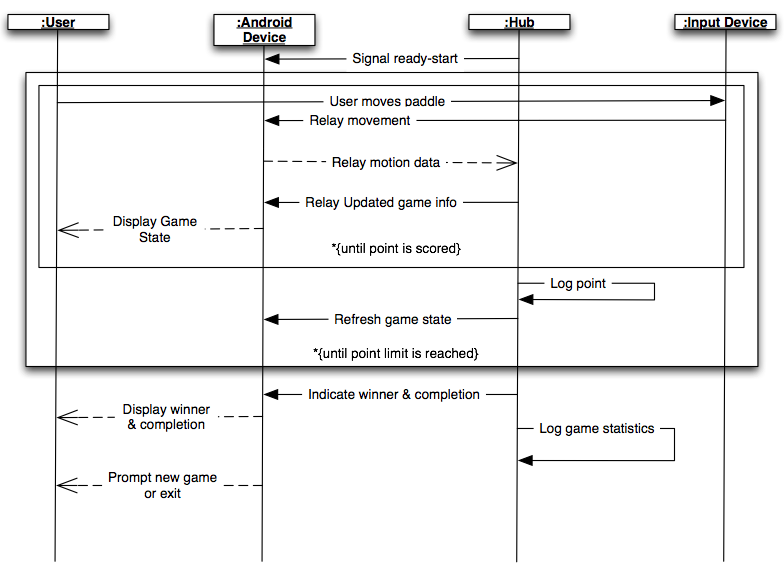
\includegraphics[scale=.5]{ssd_GamePlay_1.png}
\caption{\label{ssd_GamePlay_1}The role of our system in gameplay is described through the system sequence diagram above.}
\end{center}
\end{figure}

<<<<<<< HEAD
\textbf{Figure~\ref{ssd_GamePlay_1}} depicts the sequence of actions during a game.  The Hub signals to the Android Device that game is ready to start, then the user is able to move the paddle using their chosen Input Device.  That paddle movement is sent from the Input Device to the Android Device, which relays the motion data to the Hub.  It is then the Hub's responsibility to relay the game status back to the Android Device so that it may display the game state.  This relay of information is repeated until a point is scored.  The Hub will log the point, then refresh the game state and send this new state to the Android Device.  After a refresh, the user is able to move the paddle again and continue play.  Our system remains in this cycle until the maximum number of points is reached.  The Hub indicates the winner and completion of the game to the Android Device for informing the User.  Finally, the Hub logs the game statistics, and the Android Device prompts the User for a new game or exit.

\subsubsection*{Initializing a Game - 2.0}
=======
\textbf{Figure~\ref{ssd_GamePlay_1}} depicts the sequence of actions during a game.  The Hub signals to the Android Device that the game is ready to start, then the player is able to move the paddle using their chosen Input Device.  That paddle movement is sent from the Input Device to the Android Device, which relays the motion data to the Hub.  It is then the Hub's responsibility to relay the game status back to the Android Device so that it may display the game state.  This relay of information is repeated until a point is scored.  The Hub will log the point, then refresh the game state and send this new state to the Android Device.  After a refresh, the player is able to move the paddle again and continue play.  Our system remains in this cycle until the maximum number of points is reached.  The Hub indicates the winner and completion of the game to the Android Device, which then informs the player.  Finally, the Hub logs the game statistics and the Android Device prompts the player for a new game or exit.

\subsubsection*{Initializing a Game - v2.0}
>>>>>>> upstream/master
Actors:
\begin{itemize*}
\item Player
\item Hub
\item Device
\end{itemize*}
Preconditions:
\begin{itemize*}
\item The application is installed and open on the device.
<<<<<<< HEAD
\item The user has already created an account with Vir-Pong.
\item The input method is prepared.
=======
\item The player has already created an account with Vir-Pong.
\item The input device is tethered to the Android device and is ready to submit motion data.
>>>>>>> upstream/master
\end{itemize*}
Postconditions:
\begin{itemize*}
\item The hub is relaying game information.
\item The system is using a display to relay the game state.
\end{itemize*}
Scenario:
\begin{enumerate*}
\item \label{SelectStart}The player selects to begin a game.
\item \label{SystemPromptsAuthentication}The device prompts the player to authenticate.
\item \label{PlayerProvidesCredentials}The player provides credentials.
\item \label{SystemVerifies}The device verifies credentials with the hub.
\item \label{SystemRequestsGame}The device requests a game from the hub.
\item \label{HubSelectsOpponent}The hub selects an opponent and signals a ready-start to device.
<<<<<<< HEAD
\item \label{LoadGameState}The device loads an initial game state displayed to the user.
=======
\item \label{LoadGameState}The device loads an initial game state displayed to the player.
>>>>>>> upstream/master
\item Game begins.
\end{enumerate*}
Alternatives:\\
\ref{SelectStart}a) The player selects the wrong action.
\begin{enumerate*}
\item The player may elect to go back the the previous screen with a $return$ function.
\end{enumerate*}
\ref{PlayerProvidesCredentials}a) The player provides incorrect credentials.
\begin{enumerate*}
\item \label{HubNoAuthenticate}The device cannot authenticate into the hub.
\item The device displays a message that tells the player that the entered credentials were incorrect.
\item \label{PromptAuthenticate}The device prompts the player to authenticate.\\
Repeat \ref{HubNoAuthenticate}-\ref{PromptAuthenticate} until the Player selects the $return$ function.
\end{enumerate*}
\ref{SystemRequestsGame}a) The system can not connect to the hub.
\begin{enumerate*}
\item The device sends the player an error message that prompts the player to retry or exit.
\item Player chooses to retry.
\item System connects to hub.
\item Return to \ref{HubSelectsOpponent} of main scenario.
\end{enumerate*}
<<<<<<< HEAD
\subsubsection*{Connect to Input Device - 1.0}
Actors:
\begin{itemize*}
\item User
=======
\subsubsection*{Connect to Input Device - v1.0}
Actors:
\begin{itemize*}
\item Player
>>>>>>> upstream/master
\item Device 
\item Wii Remote
\end{itemize*}
Preconditions:
\begin{itemize*}
\item System is installed on the device and has launched.
\end{itemize*}
Postconditions:
\begin{itemize*}
\item Input device (Wii Remote) is selected and prepared for game use.
\end{itemize*}
Scenario:
\begin{enumerate*}
<<<<<<< HEAD
\item \label{BeginGame}User selects start game.
\item \label{InputMethod}System prompts user for input method: Wii Remote, device accelerometer, or touchscreen.
\item User elects to use the Wii Remote.
\item \label{ConnectWiimote}System attempts to tether Wii Remote.
\item User follows instructions from system to connect Wii Remote.
=======
\item \label{BeginGame}Player selects start game.
\item \label{InputMethod}Device prompts player for input method: Wii Remote, device accelerometer, or touchscreen.
\item Player elects to use the Wii Remote.
\item \label{ConnectWiimote}System attempts to tether Wii Remote.
\item Player follows instructions from system to connect Wii Remote.
>>>>>>> upstream/master
\item System accepts Wii Remote device and notifies user.
\item System proceeds to game launch.
\end{enumerate*}
Alternatives:\\
<<<<<<< HEAD
\ref{InputMethod}a) User selects phone accelerometer.  
\begin{enumerate*}
\item System asks user to make certain the device has an built in accelerometer.
\item User indicates that device has accelerometer.
\item System connects to device accelerometer.
\item System proceeds to game launch.
\end{enumerate*}
\ref{InputMethod}b) User selects touch screen interface.
\begin{enumerate*}
\item System asks user to touch a box displayed on-screen to ensure that a touch screen is available.
\item User touches box.
=======
\ref{InputMethod}a) Player selects phone accelerometer.  
\begin{enumerate*}
\item System asks player to make certain the device has an built in accelerometer.
\item Player indicates that device has accelerometer.
\item System connects to device accelerometer.
\item System proceeds to game launch.
\end{enumerate*}
\ref{InputMethod}b) Player selects touch screen interface.
\begin{enumerate*}
\item System asks player to touch a box displayed on-screen to ensure that a touch screen is available.
\item Player touches box.
>>>>>>> upstream/master
\item System proceeds to game launch.
\end{enumerate*}
\ref{ConnectWiimote}System attempts Wii Remote connection, and fails.
\begin{enumerate*}
\item System alerts user that connection failed.
\item Return to step \ref{InputMethod} of main scenario.
\end{enumerate*}

<<<<<<< HEAD
\subsubsection*{Changing the Game Settings - 1.0}
=======
\subsubsection*{Changing the Game Settings - v1.0}
>>>>>>> upstream/master
Actors:
\begin{itemize*}
\item Player
\item Device
\end{itemize*}
Preconditions:
\begin{itemize*}
\item The application is installed and open on the device.
\end{itemize*}
Postconditions:
\begin{itemize*}
\item The newly changed settings have been saved and will be applied to future game play.
\end{itemize*}
Scenario:
\begin{enumerate*}
<<<<<<< HEAD
\item \label{SelectChangeSettings}The player selects a $change$ $settings$ function.
\item \label{ChangeSettings}The player changes the setting(s).
\item \label{SelectSave}The player selects a $save$ $and$ $apply$ function.
\item \label{SystemSaves}The device saves changes and applies them to future game plays.
\item \label{ReturnToMainMenu}The device returns to the main menu.
=======
\item \label{SelectChangeSettings}Player selects a $change$ $settings$ function.
\item \label{ChangeSettings}Player changes the setting(s).
\item \label{SelectSave}Player selects a $save$ $and$ $apply$ function.
\item \label{SystemSaves}Device saves changes and applies them to future game plays.
\item \label{ReturnToMainMenu}Device returns to the main menu.
>>>>>>> upstream/master
\end{enumerate*}
Alternatives:\\
\ref{ChangeSettings}a) The player selects a non-valid entry for a setting.
\begin{enumerate*}
\item The device displays an error message that tells the player he entered a non-compatible value.
\item The device returns the setting to a default state.
\end{enumerate*}
\ref{SelectSave}a) The player decides not to change any settings.
\begin{enumerate*}
\item The player selects the $return$ function.
\end{enumerate*}
\onehalfspacing

\singlespacing
<<<<<<< HEAD
\subsubsection*{Viewing Stats - 1.0}
=======
\subsubsection*{Viewing Stats - v1.0}
>>>>>>> upstream/master
Actors:
\begin{itemize*}
\item Player
\item Website
\item Device
\end{itemize*}
Preconditions:
\begin{itemize*}
<<<<<<< HEAD
\item Our system is installed on the device and has launched.
\item The user has already created an account with Vir-Pong and is logged in.
\end{itemize*}
Postconditions:
\begin{itemize*}
\item The user has looked at their statistics.
\item The user can compare his to everyones.
\end{itemize*}
Scenario:
\begin{enumerate*}
\item \label{SelectStats}The player chooses view stats option
\item \label{PersonalStatRequest}The device requests personal score from website.
=======
\item Our application is installed on the device and has launched.
\item The player has already created an account with Vir-Pong and is logged in.
\end{itemize*}
Postconditions:
\begin{itemize*}
\item The player has looked at their statistics.
\item The player can compare his to everyones.
\end{itemize*}
Scenario:
\begin{enumerate*}
\item \label{SelectStats}Player chooses view stats option
\item \label{PersonalStatRequest}Device requests personal score from website.
>>>>>>> upstream/master
\item Website sends personal stats.
\item Device displays personal stats and CompareStats option.
\item \label{CompareStats}Player selects CompareStats option.
\item Device navigates to website with all player stats listed.
\item \label{Back}Player finishes viewing stats and hits back button.
\item Device returns to system state SelectStats.
\end{enumerate*}
Alternatives:\\
\ref{PersonalStatRequest}a) Unable to contact website.
\begin{enumerate*}
\item Display connection error message.
<<<<<<< HEAD
\item User may utilize a $retry$ or $continue$ button.
\item User selects $retry$.
\item Return to \ref{PersonalStatRequest}.
\end{enumerate*}

\subsubsection*{Edit Account Information}
Actors:
\begin{itemize*}
\item User
=======
\item Player may utilize a $retry$ or $continue$ button.
\item Player selects $retry$.
\item Return to \ref{PersonalStatRequest}.
\end{enumerate*}

\subsubsection*{Edit Account Information - v1.0}
Actors:
\begin{itemize*}
\item Player
>>>>>>> upstream/master
\item System
\item Vir-Pong Website
\end{itemize*}
Preconditions:
\begin{itemize*}
<<<<<<< HEAD
\item System is installed on the device and has launched.
\end{itemize*}
Postconditions:
\begin{itemize*}
\item User has edited account information.
\end{itemize*}
Scenario:
\begin{enumerate*}
\item User selects Edit Account information.
\item \label{Browser}System opens phone browser to "Vir-pong Edit Account" information page. 
\item User begins editing account information.
\item User saves and exits editing account information.
=======
\item The application is installed on the device and has launched.
\end{itemize*}
Postconditions:
\begin{itemize*}
\item Player has edited account information.
\end{itemize*}
Scenario:
\begin{enumerate*}
\item Player selects Edit Account information.
\item \label{Browser}System opens phone browser to "Vir-pong Edit Account" information page. 
\item Player begins editing account information.
\item Player saves and exits editing account information.
>>>>>>> upstream/master
\item System returns user to previous page.
\end{enumerate*} 

\onehalfspacing


%%%%%%%%%%%%%%%%%%%%%%%%%%%%%%%%
% WHAT WE HAD IN THE INITIAL REPORT:
% There are a number of key features that must function properly in order for our program
% to work on the most basic level. First, the Android device must be able to communicate with the
% Wii Remote through Bluetooth, in order to acquire accelerometer data. This function is absolutely vital
% because it allows the phone to track the position of the player and calculate the position of the
% player's paddle. After gaining data from the Wii Remote, the phone needs to pass this information
% along to a server. As the phone is sending position data, it must be able to also receive the
% position of both players' paddles and ball location from the server. In addition, the application 
% must receive information about when a point is scored, to whom the point goes to, when the game is over, and
% the final score of the players. In order to allow players to see all of this data, there must be a
% graphical representation of the game that is constantly updated by the server. Pairing down to
% essentials, this would include only a plain background, two paddles, and a ball. This GUI must
% also include a start screen that allows for players to choose to start a game and end the
% application when the game is finished.  After the completion of these primary features, we can start working
% on secondary features that are not integral to the game, but enhance the playing experience. 

%%%%%%%%%%%%%%%%%%%%%%%%%%%%%%%%%%%%%%%%%%%%%%%%%%%%%%%%%%
%4. Nonfunctional Requirements: List and briefly describe (a couple of sentences) the nonfunctional requirements for your product (you might try searching the web for FURPS to get ideas).
%%%%%%%%%%%%%%%%%%%%%%%%%%%%%%%%%%%%%%%%%%%%%%%%%%%%%%%%%%


\subsection{Usability Requirements}
%Human factors, Aesthetics, Consistency, Documentation
In order for the application to provide an experience enjoyable to a wide user base, the following usability requirements should be met:
\begin{itemize}
\item Players should have their statistics saved and then made available for viewing.
\item Players should be able to change game settings(difficulty, ball shape, etc.).
\item Users should be able to register an account through the application.
\item The application needs to be available for download via the website or on the Android Market.
\item The application should have the option to view a game in progress.
\item It would be nice to make the game environment modifiable (i.e. theming).
\item When there is not a second available human player (or connection to the hub is impossible) there should be an option for playing versus the computer in training mode.
\end{itemize}

\subsection{Reliability Requirements}
%Frequency/severity of failure, Recoverability, Predictability, Accuracy, Mean time to failure
<<<<<<< HEAD
A working product is fine, but reliability ensures a consistent experience.  With this in mind our design is striving for security of private user information and the ability to pause the game.  The latter is focused on creating a fault tolerant solution for network connectivity.  A strict testing policy will help to alleviate many other possible issues.

\subsection{Performance Requirements}
%Speed, Efficiency, Resource consumption, Throughput, Response time
The ability to adjust the display for different screens will allow for better performance of the software on different Android devices.  The system must also minimize latency when contacting the server for game information or receiving information from the Wii Remote.  No other connections are nearly as important.

\subsection{Supportability Requirements}
%Testability, Extensibility, Adaptability, Maintainability, Compatibility, Configurability, Serviceability, %Installability, Localizability, Portability
Installation, game play, and resource usage should all be properly documented in a conveniently located and navigated user-manual. A list of known compatible devices included in the manual will assist in keeping potential customers informed about our product.  There should also be some contact information for support and help when documentation is not enough.

In keeping with the project's open source roots, it will be important to make all source code well documented for the general public; make the source code readily available; give credit to non-employees with contributions; and provide substantial developer documentation. 
=======
A working product is important, but reliability ensures a consistent experience.  With this in mind, our design is striving for security of private user information and the ability to pause the game.  The latter is focused on creating a fault tolerant solution for network connectivity.  A strict testing policy will help to alleviate many other possible issues.

\subsection{Performance Requirements}
%Speed, Efficiency, Resource consumption, Throughput, Response time
The ability to adjust the display for different screens will allow for better performance of the software on different Android devices.  The system must also minimize latency when contacting the server for game information or receiving information from the Wii Remote.  There are no other connections that are quite as important.

\subsection{Supportability Requirements}
%Testability, Extensibility, Adaptability, Maintainability, Compatibility, Configurability, Serviceability, %Installability, Localizability, Portability
Installation, game play, and resource usage should all be properly documented in a conveniently located and navigated user-manual. A list of known compatible devices included in the manual will assist in keeping potential customers informed about our product.  There should also be some contact information for support and help when the available documentation is not enough.

In keeping with the project's open source roots, it will be important to make all source code well documented for the general public; make the source code readily available; give credit to non-employees that have contributed to our application; and provide substantial developer documentation. 
>>>>>>> upstream/master


\section{Domain Analysis}
%%%%%%%%%%%%%%%%%%%%%%%%%%%%%%%%%%%%%%%%%%%%%%%%%%%%%%%%%%
%5. Domain Analysis: Create a UML diagram that depicts the domain model for your product (use your fully dressed use cases as a guide but include conceptual classes that might be needed for additional features). Include a plain-english description of what is being shown in the diagram. Define any terms used in conceptual classes, attributes, or associations that might not be clear to a lay person.
%%%%%%%%%%%%%%%%%%%%%%%%%%%%%%%%%%%%%%%%%%%%%%%%%%%%%%%%%%%
<<<<<<< HEAD
\textbf{Figure~\ref{domainModel}} shows the interactions that take place and the associations involved in playing a game of virtual pong on an android device.  Throughout the game, the user controls an input device that will pass motion data to the android device.  There are three different types of input that can be used by the user: the Wii Remote, the phone accelerometer, or the touch screen interface.  The motion data from the input device is sent to the android device and immediately sent to the hub.  The hub sends back information on both the user's and an opponent's positions as well as the position of the ball.  Other relevant data is sent to and from the android device and hub, including score data and a signal that a point has been scored.  To allow the user to view their virtual pong game, the android device relies on a game interface to graphically display the constantly updating state of the game.  This game interface contains a graphical representation of two paddles and one ball that respond to information sent from the hub.
=======
\textbf{Figure~\ref{domainModel}} shows the interactions that take place and the associations involved in playing a game of Pong on an android device.  Throughout the game, the player controls an input device that will pass motion data to the android device.  There are three different types of input that can be used by the user: the Wii Remote, the phone accelerometer, or the touch screen interface.  The motion data from the input device is sent to the android device and from there is immediately sent to the hub.  The hub sends back information on both the player's and an opponent's positions as well as the position of the ball.  Other relevant data is sent to and from the android device and hub, including score data and a signal that a point has been scored.  To allow the player to view their Pong game, the android device relies on a game interface to graphically display the constantly updating state of the game.  This game interface contains a graphical representation of two paddles and one ball that respond to information sent from the hub and also keeps track of the game's current score.
>>>>>>> upstream/master
\begin{figure}
\begin{center}
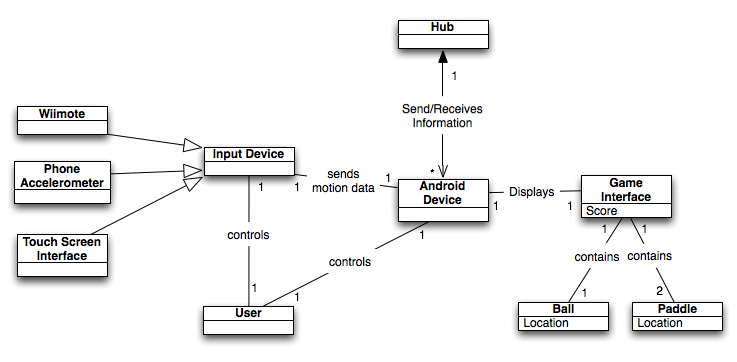
\includegraphics[scale=.7]{domainModel_Android-1.png}
\caption{\label{domainModel}Class interactions and attributes outline the major system components.}
\end{center}
\end{figure}


%%%%%%%%%%%%%%%%%%%%%%%%%%%%%%%%%%%%%%%%%%%%%%%%%%%%%%%%%%%%
%6. Implementation:
%        Include the coding style guide that your team is using. This should be fairly detailed including naming, coding conventions, and comment conventions.
%        Install documentation: include a description of all necessary procedures a developer would have to complete to install your product. If you are assuming a certain starting environment then explicitly state so (e.g. a Linux server with Apache installed). Make sure to include how the user would access and download your source code and documentation.
%        Include a current class diagram of your product
%            Diagram should depict all classes and their associations 
%        Description of algorithms, data structures and design patterns
%            Describe any complex algorithms, data structures, or design patterns your group used. Provide insights as to why you made the choices you did.
%            Describe any techniques you are using to ensure fault tolerance (e.g. if you have information to write to a db but the db is down what do you do?) 
%        Data Storage:
%            Identify all the data you are storing (ex. user athentication, medical records, back up information if the DB is down etc.)
%            If your product contains a database include both an ER Diagram and the schema for it, include a description of why you made the design decisions you did.
%            If the data is not stored in a db describe how it is stored included formatting. 
%        Describe your testing and verification procedure for your implemented code 
%%%%%%%%%%%%%%%%%%%%%%%%%%%%%%%%%%%%%%%%%%%%%%%%%%%%%%%%%%%%%%%
\section{Coding Style Guide}
The majority of the coding takes place within the $assets/www$ folder of our application.  It is, therefore, important that our team maintain a clear and concise style within this limited space.  In general, folders should be titled in the CamelCase style (first letter a capital) and individual files should be likewise with the exception that the first letter is a lower case.  Dashes may be permitted so long as it is used when there may be multiple editions of something (e.g. a "logo-blue.jpg" and "logo-red.jpg").  Further exceptions include any README files (used for build instructions) or versioned files.  

As to how many folders to have, if there exists a logical grouping between one file and several others (i.e. more than 2 files are related to one another) then these should be placed in a separate folder within the $www$ directory.  Files themselves and the code contained should follow the guidelines given below.  While these guidelines are not quite as extensive as some resources (such as Sun's own Java style guide\cite{JavaStyle-Sun}) the brevity serves our team well.

\subsection{Working with Java}
While Java is not a primary language for our team, we will be strictly following conventions laid down by Sun and other programmers\cite{JavaStyle-Sun}\cite{JavaStyle-JavaRanch}.

\subsubsection{Style Rules}
\begin{itemize}
\item All identifiers use letters ('A' through 'Z' and 'a' through 'z') and numbers ('0' through '9') only. No underscores, dollar signs or non-ascii characters (with one exception mentioned later).
\item In general, use $methodNamesLikeThis$, $variableNamesLikeThis$, $ClassNamesLikeThis$, and $SYMBOLIC\_CONSTANTS\_LIKE\_THIS$.
\item Use a separate line for an increment or decrement.
\item All fields must be private, except for some constants.
\item Class elements will follow this order: fields, constructors, methods. 
\item Limit the scope of local variables.
\item Initialize objects as late as possible.
\item Use Strings with care.
\item Avoid wrapper classes.
\end{itemize}
\textbf{A note on comments:} all methods and classes should contain a standard Javadoc comment (text description and appropriate author, version, parameter and return tags).  In-line comments are strongly encouraged to assist in readability of the code.

\subsubsection{Coding Rules}
\begin{itemize}
\item Opening curly braces should be on the same line as what they are opening.
\item Closing curly braces will be horizontally aligned with the line where the statement began.
\item Indent each time a new bracket set is created.  Indents should be four spaces.
\item All control-flow statements must use brackets.
\item Commas and semicolons are always followed by whitespace.
\item Binary operators should have a space on either side.
\item Parentheses should be used in expressions not only to specify order of precedence, but also to help simplify the expression. When in doubt, parenthesize. 
\item There will be no use of $break$.
\end{itemize}


\subsection{Working with JavaScript}
The majority of our JavaScript style guidelines are mimicked from Google\cite{JavaScriptStyle-Google}.  For further and more detailed information, see their guide.  To many new programmers, JavaScript seems very much like Java (even the name!), but it is important to note that these are different languages and we have several very different rules.

\subsubsection{Style Rules}
\begin{itemize}
\item In general, use $functionNamesLikeThis$, $variableNamesLikeThis$, $ClassNamesLikeThis$, $EnumNamesLikeThis$, $methodNamesLikeThis$, and $SYMBOLIC\_CONSTANTS\_LIKE\_THIS$.
\item Avoid using many global variables.
\item Start curly braces on the same line as what they are opening.
\item Be sure to indent blocks by four spaces.
\item Use blank lines to group logically related pieces of code.
\item Use parentheses only when required.
\item Prefer $'$ over $"$ for strings.
\item Be sure to use JSDoc comments.  A comment at the top of the file for authorship and general overview, comments for methods, and inline comments are encouraged.  The first two are done using $/*. . . */$ and the latter is $//$.
\item Use JSDoc annotations ($@priave$ and $@protected$) where appropriate.  Marking visibility is encouraged.
\item Be sure to use @param and @return tags for methods and functions.
\item Simple getters may have no description but should specify the returned values.
\end{itemize}

\subsubsection{Coding Rules}
\begin{itemize}
\item Always declare variables with $var$.
\item Use $NAMES\_LIKE\_THIS$ for constants. Use $@const$ where appropriate. Never use the $const$ keyword. 
\item Always end lines with semicolons.
\item Feel free to use nested functions but try to comment these to make them clear.
\item Do not declare functions within blocks.  Instead you may do the following:
\begin{verbatim}
if (x) {
  var foo = function() {}
}
\end{verbatim}
\item Avoid wrapper objects for primitive types.
\item The keyword $this$ is for object constructors and methods only.
\item For-in loops are only for iterating over keys in an object/map/hash.
\item Do not use multiline string literals.  Instead, use concatenation when initializing such long strings.
\item Use $onclick$ instead of $javascript:$ for anchors.
\end{itemize}

\subsection{Working with HTML5}
HTML5 and CSS are so quickly evolving of late that style guides are not readily available.  We have, however, compiled our own unique guide from some suggestions found on the Web Developer's Virtual Library\cite{HTMLStyle-WDVL}.  We recommend keeping JavaScript and CSS code in files separate from the HTML.  This is primarily to keep the code modular and sensible.  Reading HTML and JavaScript in the same file can be confusing.

\begin{itemize}
\item Block-level tags are to the far left with content indented four spaces.
\item Don't indent tags relative to their container.
\item Line up multiple attributes with the "=" signs all in the same column.
\item The home page is an index to other pages.
\item Page designs should be consistent in appearance and structure.
\item Choose a meaningful title for pages.
\item $*$Unless it is an incredibly brief code-snippet, do not include JavaScript or CSS in the $html$ file.  Place this code in a separate file.
\item Provide a $Home$ link.
\end{itemize}

\subsection{Working with CSS}
CSS doesn't normally follow any particular style guide, but we have imposed a few general rules to keep things neat\cite{CSSStyle-SmashingMagazine}.

\begin{itemize}
\item Consider a table of contents at the top of the CSS file.  This would reference labels or comments used as tags in the file.  Use a tree structure.
\item Because constants are not possible, define colors and typography used in comments at the top of the file.  This allows you to reference these colors font styles later to be consistent.  
\item Organize properties alphabetically.
\end{itemize}

\subsection{Setting up the Development Environment}
In order to develop for Android, you will need the Android SDK, the PhoneGap software, and some editor.  These pieces are relatively easy to set up, but because all systems are different, some personal configuration may be required.  All of the software mentioned below can be found, with current links, at the PhoneGap Android page\cite{PhoneGap-Android}.  

\subsubsection{Android SDK}
The Android SDK comes with an Android Emulator as well as Android libraries.
To download the SDK, first check to make sure your operating system fulfills all of the system requirements.  A list of of system requirements is available on the Android Developers website\cite{AndroidSDK-SystemRequirements}.

Next, download the Android SDK from the Android Developer website\cite{AndroidSDK-Download}.
The instructions for installation are found on the same site but on the installation page\cite{AndroidSDK-Installation}. \textbf{Note:} do not put a space in the folder name.

After that, you must add necessary components to the SDK.  The instructions for that portion are found on the components page\cite{AndroidSDK-Components}.  On your first run, you will be required to create an Android Virtual Device (AVD) that is simply a mock phone.


\subsubsection{PhoneGap}
The PhoneGap download is primarily a collection of tools that provide functionality for the HTML5 and JavaScript interface in a native application environment.  That is, the PhoneGap jar, js, and xml files all serve to support the use of HTML5 and JavaScript coding as implementing the core functionality of the application.   

\subsubsection{Editing Environment}
In theory, any development can be done from a text editor so long as you have access to the Android SDK and Java.  It is highly recommended, however, that you use Eclipse\cite{Eclipse-Helios}.  You then may want to install the ADT plugin for Android Development\cite{Eclipse-ADT}.

\subsection{Retrieving the Source}
<<<<<<< HEAD
In order to work with the source code of the project, you will likely want to use Git\cite{Github}.  Using Git, you may clone the repository from \url{git@github.com:VirPong/human-pong}.  You will then want to navigate into $Android/VirPong-Mobile/$ and create a folder called $assets$.  Navigate into $assets$ and clone \url{git@github.com:VirPong/www}.  Now you may open Eclipse and import the $VirPong-Mobile$ directory as an existing project.  You may need to point the build path to your PhoneGap Jar file (located wherever you downloaded PhoneGap and then inside the Android folder).  Once this is done, you may begin development!  \textbf{Note:} an alternative to git is to download the repository from \url{https://github.com/VirPong/human-pong} and \url{https://github.com/VirPong/www}, placing the $www$ repository in the same place mentioned above.
=======
In order to work with the source code of the project, you will likely want to use Git\cite{Github}.  Using Git, you may clone the repository from \url{git@github.com:Vir-Pong/human-pong}.  You will then want to navigate into $Android/Vir-Pong-Mobile/$ and create a folder called $assets$.  Navigate into $assets$ and clone \url{git@github.com:Vir-Pong/www}.  Now you may open Eclipse and import the $Vir-Pong-Mobile$ directory as an existing project.  You may need to point the build path to your PhoneGap Jar file (located wherever you downloaded PhoneGap and then inside the Android folder).  Once this is done, you may begin development!  \textbf{Note:} an alternative to git is to download the repository from \url{https://github.com/Vir-Pong/human-pong} and \url{https://github.com/Vir-Pong/www}, placing the $www$ repository in the same place mentioned above.
>>>>>>> upstream/master



\section{Implementation Details}
%These sections need to discuss how each piece of software works as part of the whole application.
%I have listed what I think are the important pieces to our software.

\subsection{Basic Design}
%How does PhoneGap allow us to implement a Pong game on our system?
%Where does our application interact with the pieces from other teams? (i.e. server, wii, iOS, webUI)?
The core technology of the Android application is PhoneGap\cite{PhoneGap-About}.  PhoneGap basically creates a shell on top of native devices, allowing developers to design the application using HTML5 and JavaScript.  This avoids the need to use native languages, such as Java or Objective C, and gives developers the same power used to generate content on the web.  Using PhoneGap allows us to combine with the iOS team and design a single application.  

Our application is structured such that individual "web pages" will represent different features of the application: separate pages for the home screen, game playing, settings, etc.  JavaScript files provide the functionality behind each of these features and CSS creates the styling.  The separation of the system into layout, style and functionality with specific languages allows us to use the power of languages built specifically for each piece of our whole.  While this requires a wider knowledge base, the benefits are far more important to our dedicated team.  Working with other teams' systems is made slightly easier through this choice of technology.

The WebUI and Server teams are so closely connected to internet technologies that our use of similar technologies creates a stronger basis on which to interface.  The Android application, as it stands, will not be storing any user information.  All player account and statistical information will be handled by the databases constructed by other teams.  This keeps information secure and centralized.  In the future, it may be possible that the application will hold local login information for several users, as a convenience.  

As the design of our application progresses, there may be changes to the overall implementation structure.  The current implementation, however, is designed to be rapidly prototypable and easy to work with other teams.  Going forward, we hope to keep improving on our use and understanding of the technologies at hand.


\subsection{Testing}
%How are we testing and how will we be testing our product?  This is really an incremental thing.
At this stage of development, many of our features are split across different pages of the application.  This has allowed us to test each feature in isolation.  As development progresses, we are constantly bringing new features into sections of the application we consider as $main$.  This process keeps us from breaking the functioning pieces of the system, while progressing quickly on new features.

Our general testing strategy is to use each test page as a suite of unit tests.  Buttons allow us to interact with functions and test each feature individually.  This may sound tedious, but it is effective and simulates unit testing in the best way we know.  Going forward, we will be keeping certain test pages to allow us to retest functionality.  Final builds will, of course, lack these pages.

Members of the team are encouraged to consistently bring their code to others for verification.  This keeps members informed about each other's progress, and it forces members to write cleaner, more comprehensible code.  Our ability to snapshot code into the repository has also helped in this effort.  Each snapshot is verified to be tested and functioning, with documentation marking any rough edges.  These code checks represent each end of a testing cycle.


\section{Planning and Reflection}
%%%%%%%%%%%%%%%%%%%%%%%%%%%%%%%%%%%%%%%%%%%%%%%%%%%%%%%%%%%%%%%
%7.Planning and Reflection:
%        Present a complete schedule for your project. This schedule should start from when you turned in your initial plan and project forward to the end of the project. Provide an indication of target dates and goals that were met, goals that were late, and goals that were discarded.
%        Describe major challenges that you have met thus far and how you over came them. Looking back are there things that you would have done differently.
%        Clearly indicate future milestones including dates and team member responsibilities. 
%%%%%%%%%%%%%%%%%%%%%%%%%%%%%%%%%%%%%%%%%%%%%%%%%%%%%%%%%%%%%%%
%BLAME SERVER TEAM
<<<<<<< HEAD
The biggest challenge involved with a project of this nature is the variety of interactions between all of the groups.  The Android device in particular relies on communication with the Wii Remote, server, and website, so consistent communication is vital.  Therefore, if one team manager does not make an effort to communicate, the entire project suffers.  We finally realized the importance of human communication and have planned more manager meetings for the rest of the semester.  In addition, managers have become more prompt with emailing and this has made it much easier to stay in touch and keep everyone updated on the status of the project.  Another challenge has been a general lack of motivation due to a failure to create a sense of individual accountability.  It was nearly impossible to measure how much work each individual in every group had done; consequently, team members were not highly motivated to work at a fast pace.  As a result, some teams would move ahead of the others and then feel a great deal of frustration when they had to wait for other teams to catch up.  This is an extremely difficult challenge to overcome, but the situation has improved because we are at the point where it is apparent if a team member is not contributing a satisfactory amount.  The increased manager communication also causes the group leaders to hold each other more accountable for their group’s progress.  A more specific challenge for the Android team was getting the iOS development team to agree to implement PhoneGap; this was difficult because their team members were divided on the issue.  This was especially frustrating because our team couldn’t move forward until the iOS team had made their decision.  However, we finally convinced them that the use of PhoneGap has a number of important benefits.

If we were to begin this project again, there are a number of things we would have done differently.  First of all, we would have written the APIs for Android to server and Android to Wii Remote communication at the very start of the project.  This would have allowed out team to more forward, even when the other teams were stuck.  This change would also have helped us be clearer in our expectations of what we needed from the Wii Remote team.  Another beneficial change would been restructuring the Android and iOS development teams.  Since we are using PhoneGap, the user interface for the game will be the same for both systems, so it would have been advantageous to instead divide the teams between “local” programming (the interface, pong game, features) and communications (namely between the server and the device, but also the Wii Remote to the device). 
=======
The biggest challenge involved with a project of this nature is the variety of interactions between all of the groups.  The Android device in particular relies on communication with the Wii Remote, server, and website, so consistent communication is vital.  Therefore, if one team manager does not make an effort to communicate, the entire project suffers.  We finally realized the importance of human communication and have planned more manager meetings for the rest of the semester.  In addition, managers have become more prompt with emailing and this has made it much easier to stay in touch and keep everyone updated on the status of the project.  Another challenge has been a general lack of motivation due to a failure to create a sense of individual accountability.  It was nearly impossible to measure how much work each individual in every group had done; consequently, team members were not highly motivated to work at a fast pace.  As a result, some teams would move ahead of the others and then feel a great deal of frustration when they had to wait for other teams to catch up.  This is an extremely difficult challenge to overcome, but the situation has improved because we are at the point where it is apparent if a team member is not contributing a satisfactory amount.  The increased manager communication also causes the group leaders to hold each other more accountable for their group’s progress.  A more specific challenge for the Android team was getting the iOS development team to agree to implement PhoneGap; this was difficult because their team members were divided on the issue.  This was especially frustrating because our team could not move forward until the iOS team had made their decision.  However, we finally convinced them that the use of PhoneGap has a number of important benefits for both teams.

If we were to begin this project again, there are a number of things we would have done differently.  First of all, we would have written the APIs for Android to server and Android to Wii Remote communication at the very start of the project.  This would have allowed our team to more forward, even when the other teams were stuck.  This change would also have helped us be clearer in our expectations of what we needed from the Wii Remote team.  Another beneficial change would been restructuring the Android and iOS development teams.  Since we are using PhoneGap, the user interface for the game will be the same for both systems, so it would have been advantageous to instead divide the teams between “local” programming (the interface, pong game, features) and communications (namely between the server and the device, but also the Wii Remote to the device). 
>>>>>>> upstream/master

\subsection{Past Goals}
\textbf{Thursday the 29th of September}
\begin{itemize*}
\item Complete a preliminary class diagram – Status: Completed
\item Create a prototype of the Android game interface – Status: Completed
\item Create an interface that would be compatible with both Android and iOS devices – Status: Completed 10/11 because the iOS team had not yet committed to using PhoneGap.
\item Finish Bluetooth Plugin – Status: Delayed because the Wii Remote team wished to put all of its effort into setting up the BluezIME application instead of integrating their code into the PhoneGap plugin. 
\end{itemize*}
\textbf{Thursday the 6th of October}
\begin{itemize*}
<<<<<<< HEAD
\item Server Communication to and from Android – Status: Delayed but completed 10/10.  Unforeseen difficulties were encountered during final testing.
=======
\item Server Communication to and from Android – Status: Delayed but completed 10/10 due to unforeseen difficulties that were encountered during final testing.
>>>>>>> upstream/master
\item Ability to capture wii data on interface – Status: Completed
\end{itemize*}
\textbf{Monday the 10th of October}
\begin{itemize*}
\item Commit all code and documentation to GitHub – Status: Completed
\end{itemize*}
\textbf{Thursday the 13th of October}
\begin{itemize*}
\item Create a working demo of the communication from Wii Remote to Android to server and then back to Android – Status: Completed
\item Be able to draw on Canvas – Status: Completed
\end{itemize*}
\textbf{Monday the 24th of October}
\begin{itemize*}
\item Be able to query the database from the client side to verify usernames and passwords – Status: Completed
\end{itemize*}
\textbf{Friday the 28th of October}
\begin{itemize*}
\item Finish an intermediate report for the Android team – Status: Will be completed the 28th
\end{itemize*}


\subsection{Future Goals and Deadlines}
\begin{itemize}
<<<<<<< HEAD
\item \textbf{Monday the 31st of October}: Present a working demo of the core functionality of our product.  This includes some Wii Remote to Android connectivity as well as device to server connectivity, a user interface for the phones, and a working website with a login page as well as other key features.

\item \textbf{Friday the 4th of November}: Have a more robust server connection so that the desired data is being passed from the devices to the server and back.  Also we should have a robust API for the game logic.  Both of these tasks will be handled by Jillian and Kyle.  We also will fully integrate the desired functions of BluezIME with our PhoneGap application.  Jordan and David will complete this task.

\item \textbf{Friday the 11th of November:} Start enhancing the user interface of the game.  This includes the ability to maintain and display score and sizing the paddle’s movement in relation to the device’s screen size.  Those tasked to handle this will be Kyle and David.  Jillian and Jordan will refine the user login process.

\item \textbf{Friday the 18th of November:} Allow user to select settings for their gameplay.  Kyle and Jordan will work on this task. We will also work on other secondary features such as viewing the user’s game stats and changing account information.  This will be handled by David and Jillian
=======
\item \textbf{Monday the 31st of October}: Present a working demo of the core functionality of our product.  This includes some Wii Remote to Android connectivity as well as Android to server connectivity, a user interface for the phones, and a working website with a login page as well as other key features.

\item \textbf{Friday the 4th of November}: Have a more robust server connection so that the desired data is being passed from the devices to the server and back.  Also we should have a robust API for the game logic.  Both of these tasks will be handled by Jillian and Kyle.  We also will fully integrate the desired functions of BluezIME with our PhoneGap application.  Jordan and David will complete this task.

\item \textbf{Friday the 11th of November:} Start enhancing the user interface of the game.  This includes the ability to maintain and display score and sizing the paddles' movement in relation to the device’s screen size.  Those tasked to handle this will be Kyle and David.  Jillian and Jordan will refine the user login process.

\item \textbf{Friday the 18th of November:} Allow the player to select settings for their game play.  Kyle and Jordan will work on this task. We will also work on other secondary features such as viewing the player’s game stats and changing account information.  This will be handled by David and Jillian
>>>>>>> upstream/master

\item \textbf{Tuesday the 25th of November:} Clean up and embellish the application’s user interface and test the game a great deal.  We will all help in both of these activities. 

\item \textbf{Friday the 2nd of December:} Have all core functionality completed and satisfactorily tested.  Have as many secondary features completed and tested as possible.  Make sure all documentation is complete and the code follows our style guides. 

\item \textbf{Friday the 9th of December:} Code freeze.  Begin pulling together the components for our final product presentation.

\item \textbf{Wednesday the 14th of December:}  Present our product to management.
\end{itemize}


%%%%%%%%%%%%%%%%%%%%%%%%%%%%%%%%%%%%%%%%%%%%%%%%%%%%%%%%%%%%%%%
%8. References: Clearly indicate all the tools and sources you have used in the development of your product thus far. 
%%%%%%%%%%%%%%%%%%%%%%%%%%%%%%%%%%%%%%%%%%%%%%%%%%%%%%%%%%%%%%%

\newpage
\bibliographystyle{amsplain}
\bibliography{intermediateReport.Android.bib}

















\end{document}
